\documentclass[12pt]{article}

% ---------- Encoding & fonts ----------
\usepackage[utf8]{inputenc}
\usepackage[T1]{fontenc}
\usepackage{microtype}
\usepackage{newtxtext,newtxmath}

% ---------- Page & core ----------
\usepackage[a4paper,margin=1in]{geometry}
\usepackage{setspace}
\usepackage{titling}
\usepackage{titlesec}
\usepackage{tocloft}
\usepackage{tabularx}
\usepackage{longtable} % <-- MUST be here (preamble)
\usepackage{array}
\usepackage{booktabs}
\usepackage{enumitem}
\usepackage{float}
\usepackage{ragged2e}
\usepackage{graphicx}
\usepackage{etoolbox} % robust section hook

\newcolumntype{Y}{>{\RaggedRight\arraybackslash}X}

% ---------- Section heading style ----------
\titleformat{\section}{\bfseries\Large}{\thesection.}{0.6em}{\bfseries}
\titlespacing*{\section}{0pt}{*1.2}{*0.6}
\titleformat{\subsection}{\bfseries\normalsize}{\thesubsection.}{0.5em}{\bfseries}
\titlespacing*{\subsection}{0pt}{*0.9}{*0.4}
\titleformat{\subsubsection}{\bfseries}{\thesubsubsection.}{0.5em}{\bfseries}
\titlespacing*{\subsubsection}{0pt}{*0.7}{*0.3}

% ---------- Start each major section on a new page (robust) ----------
\pretocmd{\section}{\clearpage}{}{}

% ---------- TOC look ----------
\renewcommand{\contentsname}{Table of Contents}
\renewcommand{\cfttoctitlefont}{\bfseries\large}
\renewcommand{\cftdotsep}{1}
\setlength{\cftbeforesecskip}{2.5pt}
\setlength{\cftbeforesubsecskip}{1.5pt}
\renewcommand{\cftsecpagefont}{\normalfont}
\renewcommand{\cftsubsecpagefont}{\normalfont}
\renewcommand{\cftsubsubsecpagefont}{\normalfont}
\setcounter{tocdepth}{3}

% ---------- Hyperlinks & bookmarks (robust) ----------
\usepackage[unicode,psdextra]{hyperref}
\usepackage{bookmark} % load right after hyperref
\hypersetup{
  hidelinks,
  bookmarksopen=true,
  bookmarksnumbered=true,
  hypertexnames=false, % <-- fixes duplicate "page." destination warnings
  pdfauthor={CSULA Team Sun-1},
  pdftitle={System Requirements Specification}
}

% ---------- Page Numbering ----------
\usepackage{fancyhdr}
\pagestyle{fancy}
\fancyhf{}                    % clear header and footer
\fancyfoot[C]{\thepage}       % page number centered at bottom
\renewcommand{\headrulewidth}{0pt}
\renewcommand{\footrulewidth}{0pt}

\begin{document}

% ===================== Title page =====================
\pagenumbering{gobble}

\begin{titlepage}
\centering
\vspace*{3cm}

% Top title
{\LARGE \textbf{Software Requirements Specification}\par}
\vspace{1.5cm}

% "for" line
{\large for\par}
\vspace{1cm}

% Project title
{\LARGE \textbf{Employee Performance Review (EPR) Dashboard}\\
\LARGE \textbf{and Workflow System}\par}
\vspace{1.5cm}

% Version line
{\normalsize Version 0.2 Approve Pending\par}
\vspace{2cm}

% Prepared by + names
{\normalsize Prepared by:\par}
\vspace{0.8cm}
{\normalsize
Alyssa Arroyo\\
Momoka Aung\\
Chiemela Eziechile-Nwoke\\
Hari Ram Gurung\\
Michael Hareu\\
Hoang Le\\
John Lopez\\
Aidan McBride\\
Luis Morales\\
James San\\
Hayk Vardapetyan\par}
\vspace{2cm}

% Affiliations
{\normalsize Santa Barbara County Public Defender’s Office\par}
{\normalsize California State University, Los Angeles\par}

% Push date to bottom
\vfill
{\normalsize 03 December 2025\par}

\clearpage
\pagenumbering{arabic}

\end{titlepage}

% ===================== TOC =====================
\addcontentsline{toc}{section}{Table of Contents}
\begingroup
\singlespacing
\setlength{\parskip}{0pt}
\setlength{\parindent}{0pt}
\pagenumbering{arabic}
\tableofcontents
\endgroup
\newpage

% ===================== Revision History =====================
\section*{Revision History}
\addcontentsline{toc}{section}{Revision History}

\renewcommand{\arraystretch}{1.3}
\begin{center}
\begin{tabular}{|p{2cm}|p{3cm}|p{3.5cm}|p{7cm}|}
\hline
\textbf{Version} & \textbf{Date} & \textbf{Author} & \textbf{Reason for Changes} \\ \hline
1.0 & 08 Sep 2025 & Momoka Aung, Chiemela Eziechile - Nwoke & Initial draft created. \\ \hline
1.1 & 16 Oct 2025 & Momoka Aung & Added structure, clarified roles, and incorporated high-level requirements. \\ \hline
1.2 & 24 Oct 2025 & Momoka Aung & Expanded details per feedback; separated EPR workflow from Power BI section; added field lists, triggers, mappings, and KPI definitions. \\ \hline
1.3 & 21 Nov 2025 & Momoka Aung & Updated with Personnel Matters project information. \\ \hline
1.4 & 3 Dec 2025 & Momoka Aung & Added workflow diagram. \\ \hline
1.5 & 30 Jan 2026 & Momoka Aung & Added information of Recruitments, Vacancies, and Separation projects.  \\ \hline
1.6 & 13 Mar 2026 & Momoka Aung & Finalized draft  \\ \hline
\end{tabular}
\end{center}


% ===================== 1. Introduction =====================
\section{Introduction}

This Software Requirements Specification (SRS) describes the key features and expectations for the Human Resources Workflow Management System, which includes both the Employee Performance Review (EPR), the Personnel Matters, Recruitments/Vacancies, and Separation Tracker and Dashboard projects. The system is being developed for the Santa Barbara County Public Defender’s Office to improve how HR processes are tracked, managed, and reported.

This document outlines what the system should do, how it should perform, and the standards it must meet. It serves as a shared reference for HR staff, project stakeholders, and developers to ensure a clear understanding of the project’s goals, scope, and overall framework.

\subsection{Purpose}

This Software Requirements Specification (SRS) defines the functional and nonfunctional requirements for the Human Resources Workflow Management System, which includes the Employee Performance Review (EPR), the Personnel Matters, Recruitments/Vacancies, and Separation Tracker and Dashboard projects. 

The purpose of these system is to automate and centralize HR workflows across all divisions of the Santa Barbara County Public Defender’s Office, improving how performance reviews, employee concerns, and related documentation are tracked and completed. The system ensures timely follow-up and accountability through automated reminders, escalation notifications, and structured data management. It replaces current manual, email-based processes with a transparent, repeatable, and auditable workflow that uses Smartsheet for process automation and Box for secure document storage.

\subsection{Intended Audience and Reading Suggestions}

\begin{itemize}
  \item \textbf{HR Staff \& Product Owner:} Configure schedules, templates, and monitor compliance (Sections 1–2, 4).
  \item \textbf{Supervisors \& Division Leads:} Manage review workflows and respond to reminders (Sections 2–4).
  \item \textbf{Developers / Integrators:} Implement Smartsheet automations, email notifications, Box integration, and develop the AWS architecture and APIs supporting Smartsheet and Box.com integrations (Sections 3–4).
  \item \textbf{QA / Reviewers \& IT Security:} Verify system behavior and ensure policy alignment (Sections 4–6).
\end{itemize}

\subsection{Product Scope}

The Human Resources Workflow Management System is designed to modernize and centralize four key HR functions within the Santa Barbara County Public Defender’s Office: the Employee Performance Review (EPR), the Personnel Matters, Recruitments/Vacancies, and Separation Tracker and Dashboard projects. Together, these systems streamline HR processes, reduce manual workload, and improve transparency and accountability across all divisions.

The \textbf{Employee Performance Review (EPR) Tracker} will automate the end-to-end review process. It tracks due dates, sends automated reminder and escalation notifications, and records completion status in a centralized Smartsheet dashboard. Data from the tracker will also feed into Power BI dashboards to provide real-time reporting, analytics, and leadership visibility into review progress and compliance. Supervisor(s) and manager(s) complete and review EPR templates, while the EPR Tracker Workflow uploads finalized documents to the secured Box repository, where they are stored and linked to corresponding tracker entries. The EPR component ensures that reviews are completed on time, properly documented, and easily accessible for compliance and reporting purposes.

The \textbf{Personnel Matters Tracker} will provide a structured process for recording, tracking, and resolving employee-raised concerns such as disputes, investigations, or disciplinary actions. It introduces standardized intake forms for both employees and HR staff, metadata tracking (status, due dates, responsible parties), and integrated document management through Box. Data from the tracker will also feed into Power BI dashboards, providing real-time reporting, analytics, and visibility into review progress and compliance. This component replaces informal, email-based submissions with a consistent, auditable workflow that improves recordkeeping and communication between HR and management.

The \textbf{Vacancies \& Recruitment Tracker} will provide a centralized process for tracking open positions, recruitment activity, and hiring outcomes across the organization. It introduces a standardized vacancy tracker that captures key data elements such as job class, department, funding status, vacancy start date, recruitment stage, interview activity, and time-to-hire metrics. Integrated analytics through Power BI deliver real-time visibility into active vacancies, recruitment progress, new hires, and internal versus external recruitment trends.

This component replaces the current manual process of downloading vacancy reports from the County’s Den application in PDF or Excel format and re-entering data into tracking sheets. By consolidating vacancy management into a structured, continuously maintained system, the dashboard improves data consistency, reporting accuracy, and workforce planning visibility for HR and leadership.

The \textbf{Separations Dashboard} provides a centralized process for recording and tracking employee exits. HR begins the process by filling out the designated Smartsheet form with  the leaving employee’s information, including position details, reason for exit, effective date, and last working day. Required fields help ensure data accuracy and completeness. The system generates standardized separation notifications and tracks their status. A Power BI dashboard displays separation trends by division, job class, and reason for exit to support reporting and workforce planning.

This component replaces informal, email-based processes with a consistent, auditable workflow secured through SmartSheet's Single Sign-On (SSO), improving transparency and reporting accuracy.


Those components share a unified data model, common user interface, and secure authentication through Single Sign-On (SSO). The system provides HR with real-time visibility into active cases, overdue tasks, and historical records, ultimately improving process efficiency, compliance with county policies, and data accuracy.

\subsection{Definitions, Acronyms, and Abbreviations}

\begin{itemize}
  \item \textbf{EPR:} Employee Performance Review
  \item \textbf{HR:} Human Resources
  \item \textbf{Smartsheet:} Workflow and tracking platform used for automation and status management
  \item \textbf{Box:} County-secured document repository for finalized HR records
  \item \textbf{Power BI:} Business intelligence and reporting platform used to create dashboards and analytics visualizations
  \item \textbf{SSO:} Single Sign-On for authenticated access
  \item \textbf{Personnel Matters:} HR cases related to employee disputes, investigations, or disciplinary actions
\end{itemize}

\subsection{References}

\begin{itemize}
  \item \href{https://cosantabarbara.app.box.com/s/xzxniv8dk6gt2eormc0b8ihsn686cf6l}{Project Overview: Box Link}
\end{itemize}

% ===================== 2. Overall Description =====================
\section{Overall Description}

This section provides a high-level overview of the Human Resources Workflow Management System, which includes the Employee Performance Review (EPR), Personnel Matters Tracker, Vacancies and Recruitment Tracker, and Separation Tracker and Dashboard. Together, these components provide a centralized and structured approach to managing key HR processes.

\subsection{System Analysis}

The Human Resources Workflow Management System is designed to simplify how the Public Defender’s Office manages core HR processes, including Employee Performance Reviews (EPR), Personnel Matters, Vacancies and Recruitments, and Employee Separations. Currently, these processes rely on spreadsheets, email communication, and manual downloads from external applications, making it difficult to track progress, ensure timely completion, and maintain consistent documentation.

By consolidating these workflows into a centralized platform, the system standardizes how HR activities are recorded, routed, and monitored. Automated notifications, structured tracking, and integrated dashboards provide clearer visibility into deadlines, case status, hiring activity, and separation trends. This allows HR staff to manage tasks more efficiently while giving leadership real-time insight into workforce operations.

The goal of the system is to improve accountability, reduce administrative burden, and enhance reporting accuracy across all HR functions. Key challenges include designing reliable workflow automation, ensuring secure document management, and maintaining compliance with County data privacy and retention standards. By leveraging a centralized workflow and reporting architecture, the system provides a consistent, auditable, and secure solution tailored to the office’s operational needs.

\subsection{Product Perspective}

The Human Resources Workflow Management System enhances the Public Defender’s Office’s existing HR processes by integrating with County enterprise platforms to streamline workforce operations. By centralizing performance reviews, personnel matters, recruitment tracking, and separations into a unified workflow environment, the system improves accessibility, accountability, and reporting consistency.

The solution integrates with key County-supported tools:

\begin{itemize}
  \item \textbf{Smartsheet:} Provides the structured workflow environment for tracking HR activities, managing review timelines, routing approvals, and maintaining case records.
  \item \textbf{Box:} Serves as the secure repository for finalized HR documents and supporting records.
  \item \textbf{Email System:} Enables automated notifications and reminders for workflow actions, approvals, and deadlines.
  \item \textbf{Amazon Web Services (AWS):} Provides cloud infrastructure, backend services, and API integrations supporting the system’s workflows, data processing, and secure connectivity with Smartsheet and Box.
  \end{itemize}

In addition, the system includes a cloud-based automation service implemented using AWS Services such as AWS Lambda, written in the Python programming language. This service manages cross-system operations such as
sending outbound emails with Box-hosted documents and executing controlled workflow updates.

By leveraging these existing platforms through secure Single Sign-On (SSO), the system eliminates reliance on fragmented spreadsheets and email-based tracking. Employees and HR staff can manage tasks, monitor progress, and access records within a consistent cloud-based environment aligned with the County’s IT infrastructure. This integrated approach improves operational efficiency while maintaining compliance with County security and data retention standards.

\subsection{Product Functions}

The EPR Dashboard and Workflow System provides four primary functions that work together to streamline the review process:

\begin{itemize}
  \item \textbf{2.3.1 EPR Tracking and Scheduling}
  \begin{itemize}
    \item Maintain a centralized Smartsheet tracker that lists all active employees, their supervisors, review periods, and due dates.
    \item Automatically calculate next review dates based on prior completion records.
    \item Send automated reminder emails 60, 30, 14, and 7 days before/after a review is due.
    \item Escalate overdue reviews to division leads at 7 days past due, and to department heads at 14 days past due.
    \item Log all reminder and escalation events in Smartsheet for audit purposes.
  \end{itemize}

  \item \textbf{2.3.2 Offline Review and Submission}
  \begin{itemize}
    \item Allow supervisors to complete EPR forms offline using HR-provided templates.
    \item Upload finalized documents to Box and link the file URL in Smartsheet for record-keeping.
  \end{itemize}

\item \textbf{2.3.3 Personnel Matters Case Tracking}
  \begin{itemize}
    \item Maintain a structured Smartsheet tracker for employee-submitted concerns, investigations, and HR actions.
    \item Include intake forms for both employees and HR staff, with required metadata (status, next-step due dates, responsible HR personnel).
    \item Enable document uploads and Box linkage for supporting evidence or finalized outcomes.
    \item Provide HR with real-time dashboards summarizing open, in-progress, and closed cases.
  \end{itemize}
  
    \item \textbf{2.3.4 Vacancies and Recruitments Tracking}
  \begin{itemize}
    \item Maintain a centralized Smartsheet tracker for all active vacancies and recruitment efforts.
    \item Support initial data population through uploads from the county-provided Den application, with manual updates by HR as recruitment progresses.
    \item Capture standardized recruitment data including position ID, job class, office location, recruitment status, funding status, vacancy start date, date filled, and time-to-hire.
    \item Feed structured data into a Power BI dashboard to provide leadership with real-time visibility into active vacancies, recruitment status, new hires, interview activity, and historical hiring trends.
  \end{itemize}

  \item \textbf{2.3.5 Employee Separations Tracking and Reporting}
  \begin{itemize}
    \item Maintain a centralized Smartsheet tracker to record employee separation data, including staff information, position details, job class, reason for exit, submission date, and last working day.
    \item Automate field dependencies to reduce manual data entry and improve accuracy.
    \item Utilize a standardized intake form to validate required fields and ensure all minimum necessary information is captured for accurate and efficient processing.
    \item Trigger standardized separation notification emails using data captured in Smartsheet.
    \item Provide Power BI dashboards that summarize separations by job class and exit reason, with configurable time-based filters for leadership reporting.
  \end{itemize}
\end{itemize}

By integrating these functions into a single system, the Dashboards reduce administrative effort, ensures policy compliance, and provides supervisors and HR with clear, up-to-date visibility into the review process.

\subsection{User Classes and Characteristics}
\begin{longtable}{@{}p{4.2cm}p{3.2cm}p{6.2cm}@{}}
\toprule
\textbf{Role} & \textbf{Access Scope} & \textbf{Typical Actions} \\
\midrule
Supervisor & Team-only & Initiate/approve EPRs; respond to reminders \\
HR Staff (Data Stewards) & Department-wide & Configure automations/templates; monitor compliance; manage data quality \\
Division Lead & Division & Review escalations; enforce deadlines \\
Head of Office & Org-wide & Final approvals; view executive dashboards \\
Admin / IT & Org-wide & SSO, permissions, integration health \\
\bottomrule
\end{longtable}

\subsection{Operating Environment}

The system operates within the following environment:

\begin{itemize}
    \item Cloud-based deployment using the County’s enterprise licenses for Smartsheet and Box.
    \item Accessible through modern web browsers, including Google Chrome, Microsoft Edge, and Mozilla Firefox.
    \item Requires an active internet connection and County Single Sign-On (SSO) credentials.
    \item Supported on both desktop and mobile devices; administrative configuration is primarily performed on desktop browsers.
    \item Integrated with County email services (Microsoft Outlook/Exchange) for automated reminders and notifications.
    \item Access restricted to authorized employees, supervisors, HR staff, and administrators, with role-based permissions defined for each workflow (EPR, Personnel Matters, Vacancies and Recruitments, and Separations).
\end{itemize}

% --------------------------------------------------

\subsection{Design and Implementation Constraints}

The system is subject to the following constraints:

\begin{itemize}
    \item Must comply with Santa Barbara County IT policies, data privacy standards, and records retention regulations.
    \item Development and deployment must be completed within the academic semester timeline.
    \item User permissions and automation capabilities are limited by the County’s administrative configurations within Smartsheet and Box enterprise accounts.
    \item System performance may vary depending on device capability and network speed.
    \item The design must prioritize reliability, security, and maintainability to ensure long-term compliance with County operational policies.
\end{itemize}

\subsection{User Documentation}

The Human Resources Workflow Management System will provide multiple user documentation resources to support onboarding and ongoing use. This Software Requirements Specification (SRS) will serve as a reference guide for understanding the system’s purpose and functionality.

A user guide and quick reference materials will be provided to assist HR staff and supervisors in navigating dashboards, managing workflows, and accessing reports. A live demonstration during the project presentation will introduce users to the system’s core features, including workflow tracking, automated notifications, and reporting capabilities.

All documentation will be distributed in PDF format and stored in a shared County repository to ensure accessibility and version control.

\subsection{Assumptions and Dependencies}

The system is based on the following assumptions and dependencies:

\begin{itemize}
    \item The Santa Barbara County Single Sign-On (SSO) system remains active and available for user authentication to Smartsheet and Box.
    \item HR maintains an up-to-date supervisor–employee hierarchy to ensure accurate routing of reminders and escalations.
    \item Users have stable internet connectivity and access to County-approved browsers and hardware.
    \item Smartsheet enterprise automation features (including date-based reminders and escalation workflows) remain available under the County’s licensing plan.
    \item Box continues to serve as the official repository for finalized documents, with sufficient storage capacity and retention policy compliance.
    \item Changes to County IT infrastructure, security protocols, or access permissions may require updates to automation rules or system configurations.
\end{itemize}

\subsection{Apportioning of Requirements}

System functionality will be implemented in phases as follows:

\begin{itemize}
    \item \textbf{Phase 1:} Implementation of the Employee Performance Review (EPR) workflow, including centralized tracking, automated reminders and escalations, reporting dashboards, and secure document storage.
    
    \item \textbf{Phase 2:} Implementation of the Personnel Matters workflow, including structured intake forms, case tracking, status management, and document storage.
    
    \item \textbf{Phase 3:} Implementation of the Vacancies and Recruitments workflow, including centralized vacancy tracking and recruitment reporting.
    
    \item \textbf{Phase 4:} Implementation of the Employee Separations workflow, including separation tracking, notification management, and reporting.
\end{itemize}

Each phase may be deployed independently but will operate within the same centralized system architecture.

% ===================== 3. External Interface Requirements =====================
\section{External Interface Requirements}

This section describes how the system interacts with external interfaces, including user interfaces, hardware, software, and communication services within the Santa Barbara County Public Defender’s Office IT environment.

% --------------------------------------------------

\subsection{User Interfaces}

The system shall provide the following user interface capabilities:

\begin{itemize}
    \item A user-friendly interface within Smartsheet that allows HR staff and supervisors to view, update, and manage workflow records.
    
    \item Structured Smartsheet forms for entering and updating data such as employee information, review periods, due dates, case status, responsible parties, and document links.
    
    \item Visual dashboards summarizing workflow progress, including counts of records by status (e.g., Not Started, In Progress, Completed, Overdue).
    
    \item Clear visual indicators (e.g., color coding or status flags) to highlight overdue or pending items.
    
    \item Organized document access within Box using structured folders and metadata for finalized records.
    
    \item Accessible interfaces that support screen readers and high-contrast viewing options.
    
    \item Clear labels, tooltips, and validation messages to guide users during data entry and updates.
    
    \item Embedded help links providing access to user guides and FAQs.
\end{itemize}

% --------------------------------------------------

\subsection{Hardware Interfaces}

The system operates entirely in a cloud-based environment and does not require dedicated hardware. Users may access the system through County-approved desktop computers, laptops, or mobile devices with internet connectivity. No local installation or specialized equipment is required.

% --------------------------------------------------

\subsection{Software Interfaces}

The system integrates with the following County-supported software platforms:

\begin{itemize}
    \item \textbf{Smartsheet} — Workflow management and structured data tracking.
    \item \textbf{Box} — Secure document storage and retrieval.
    \item \textbf{Microsoft Outlook/Exchange} — Automated email notifications and reminders.
    \item \textbf{Power BI} — Reporting dashboards and analytics visualization.
\end{itemize}

In addition, the system utilizes a cloud-based automation service to support advanced workflow processing, including outbound email handling and document synchronization between platforms.

All integrations use supported, secure connections and comply with County IT policies. No unsupported third-party applications are required.

% --------------------------------------------------

\subsection{Communications Interfaces}

All system communications shall:

\begin{itemize}
    \item Use encrypted HTTPS/TLS 1.2 or higher protocols.
    \item Authenticate users through the County Single Sign-On (SSO) system.
    \item Transmit automated notifications via the County’s Microsoft Exchange network.
\end{itemize}

All communications must comply with County data security and privacy standards.

% ===================== 4. Requirements Specification =====================
\section{Requirements Specification}

The Requirements Specification section defines the system’s functional capabilities and expected behaviors across all HR workflow modules.

% --------------------------------------------------
\subsection{Functional Requirements}

% --------------------------------------------------
\subsubsection{EPR Workflow}

\begin{enumerate}
    \item The system shall maintain employee records containing review-related information, including employee number, name, job class, start date, employment status, probation due date, and signed EPR due date.
    
    \item The system shall track previous review completion dates and historical review status.
    
    \item The system shall allow HR to initiate a new review cycle.
    
    \item The system shall route reviews sequentially through assigned supervisors and leadership for approval.
    
    \item The system shall display the current stage of each review.
    
    \item The system shall prevent progression to the next stage until the current stage is completed.
    
    \item The system shall archive finalized reviews in a secure document repository.
    
    \item The system shall record a link to the archived document.
    
    \item The system shall prepare the record for the next review cycle upon completion.
\end{enumerate}

% --------------------------------------------------
\subsubsection{Personnel Matters Workflow}

\begin{enumerate}
    \item The system shall allow employees and HR staff to submit personnel matter information using a structured intake form.
    
    \item Upon submission of the form, the system shall create a new case record within the Personnel Matters tracker.
    
    \item The system shall allow HR to update case status, assign responsible parties, and record outcomes.
    
    \item The system shall require documentation of outcome before a case can be marked as closed.
    
    \item The system shall restrict case access based on user role.
    
    \item The system shall support reporting on open, in-progress, and closed cases.
\end{enumerate}

% --------------------------------------------------
\subsubsection{Vacancies and Recruitment Workflow}

\begin{enumerate}
    \item The system shall allow HR to upload vacancy or recruitment data files exported from the County’s Den application.
    
    \item Upon successful upload, the system shall create or update vacancy records within the Vacancies and Recruitment tracker.
    
    \item The system shall allow HR to update recruitment status as positions progress.
    
    \item The system shall track interview activity and hiring outcomes.
    
    \item The system shall identify positions as filled or on hold.
    
    \item The system shall support reporting of recruitment metrics and trends.
\end{enumerate}

% --------------------------------------------------
\subsubsection{Employee Separation Workflow}

\begin{enumerate}
    \item The system shall allow HR staff to submit employee separation information using a structured form.
    
    \item Upon submission, the system shall create a new separation record in the Separation tracker.
    
    \item The system shall enforce completion of required separation fields before finalization.
    
    \item The system shall generate standardized separation notifications.
    
    \item The system shall track notification status.
    
    \item The system shall support reporting of separation trends and metrics.
\end{enumerate}

% --------------------------------------------------
\subsection{External Interface Requirements}

This section defines how the system interacts with external platforms and services used by the Santa Barbara County Public Defender’s Office.

\begin{itemize}
    \item 4.2.1 The system shall interface with a web browser to allow HR staff, supervisors, and administrators to access the workflow dashboards.

    \item 4.2.2 The system shall interface with \textbf{Smartsheet} to manage workflow records, including Employee Performance Reviews, Personnel Matters, Vacancies and Recruitment tracking, and Employee Separations.

    \item 4.2.3 The system shall interface with \textbf{Box} to store finalized documents and provide secure document access links.

    \item 4.2.4 The system shall interface with \textbf{Microsoft Outlook/Exchange} to send automated notifications, reminders, and escalation messages.

    \item 4.2.5 The system shall interface with \textbf{Power BI} to generate dashboards and analytics reports for leadership.

    \item 4.2.6 The system shall interface with a cloud-based automation service to support workflow tasks such as document handling and automated email processing.
\end{itemize}

% --------------------------------------------------
\subsection{Logical Data Requirements}

This section describes how system data is stored and managed across integrated platforms.

\begin{itemize}
    \item 4.3.1 The system shall store workflow records within Smartsheet trackers for EPRs, Personnel Matters, Vacancies and Recruitments, and Employee Separations.

    \item 4.3.2 The system shall store finalized documents within Box using secure links referenced in Smartsheet records.

    \item 4.3.3 The system shall ensure that stored data complies with Santa Barbara County data security and retention policies.

    \item 4.3.4 The system shall support structured datasets for reporting and analytics dashboards.
\end{itemize}

% --------------------------------------------------
\subsection{Design Constraints}

This section outlines technical and operational constraints affecting the system design.

\begin{itemize}
    \item 4.4.1 The system shall be accessed through modern web browsers by authorized users.

    \item 4.4.2 User authentication shall be managed through the County Single Sign-On (SSO) system.

    \item 4.4.3 System availability depends on the uptime and performance of Smartsheet, Box, Power BI, and related cloud services.

    \item 4.4.4 The system must comply with Santa Barbara County data privacy, security, and records retention policies.

    \item 4.4.5 System functionality may be limited by the capabilities and licensing constraints of the integrated enterprise platforms.
\end{itemize}

% ===================== 5. Other Nonfunctional Requirements =====================
\section{Other Nonfunctional Requirements}

\subsection{Performance Requirements}

Performance requirements define how efficiently the system must operate under normal conditions.

\begin{itemize}
    \item 5.1.1 The system shall support concurrent user sessions without noticeable performance degradation.
    \item 5.1.2 The system shall process automated notifications and workflow updates promptly after scheduled triggers.
    \item 5.1.3 The system shall handle a significant volume of HR records and dashboard queries within acceptable response times.
    \item 5.1.4 The system should recover from service interruptions within a reasonable timeframe to minimize disruption.
\end{itemize}

% --------------------------------------------------

\subsection{Safety Requirements}

This section outlines measures that protect system stability and data integrity.

\begin{itemize}
    \item 5.2.1 The system shall prevent data corruption during automation failures or partial updates.
    \item 5.2.2 The system shall allow restoration of document versions through supported platform features.
    \item 5.2.3 The system shall follow County backup and data retention policies.
\end{itemize}

% --------------------------------------------------

\subsection{Security Requirements}

This section defines security and access control standards.

\begin{itemize}
    \item 5.3.1 The system shall require authentication through County Single Sign-On (SSO).
    \item 5.3.2 The system shall enforce role-based access control (RBAC).
    \item 5.3.3 Sensitive documents shall be stored in a secure repository.
    \item 5.3.4 The system shall comply with County data privacy and information security policies.
    \item 5.3.5 Reporting dashboards shall restrict data visibility based on user role.
\end{itemize}

% --------------------------------------------------

\subsection{Software Quality Attributes}

This section specifies quality characteristics necessary for long-term effectiveness.

\begin{itemize}
    \item 5.4.1 The system shall provide an intuitive and user-friendly interface.
    \item 5.4.2 The system shall maintain high availability during County business hours.
    \item 5.4.3 System configurations and automations shall be documented for maintainability.
    \item 5.4.4 The system should support future workflow expansions without major redesign.
\end{itemize}

% --------------------------------------------------

\subsection{Business Rules}

This section defines operational policies governing system use.

\begin{itemize}
    \item 5.5.1 Each employee shall complete one formal performance review annually unless otherwise specified by HR policy.
    \item 5.5.2 Only authorized HR personnel may create or close personnel matter records.
    \item 5.5.3 Only administrators shall configure system settings and automation rules.
    \item 5.5.4 Standard users shall not delete official HR records.
    \item 5.5.5 Access to workflow data shall be determined by user role.
\end{itemize}


% ===================== 6. Legal and Ethical Considerations =====================
\section{Legal and Ethical Considerations}

\subsection{Privacy and Security}

The system shall operate in compliance with Santa Barbara County legal, privacy, and security standards. The following requirements apply:

\begin{itemize}
    \item 6.1.1 The system shall comply with all applicable County HR policies, data privacy regulations, and records retention requirements.
    
    \item 6.1.2 The system shall ensure that all performance review, personnel matter, recruitment, and separation data is securely collected, stored, and processed.
    
    \item 6.1.3 Access to data shall follow the principle of least privilege, restricting users to only the information necessary for their assigned role.
    
    \item 6.1.4 Personally identifiable information (PII) shall be protected through secure authentication, role-based access control, and encrypted data transmission.
    
    \item 6.1.5 The system shall maintain audit logs of user actions and document access to support accountability and compliance reviews.
    
    \item 6.1.6 All inter-system data transfers shall use encrypted HTTPS/TLS 1.2 or higher protocols.
\end{itemize}

% --------------------------------------------------

\subsection{Ethical Considerations}

The system shall promote responsible and ethical handling of employee data.

\begin{itemize}
    \item 6.2.1 Employee performance and personnel data shall be used solely for authorized HR and administrative purposes.
    
    \item 6.2.2 The system shall support transparency by clearly documenting workflows and data handling practices.
    
    \item 6.2.3 Workflows shall promote fairness, consistency, and impartial treatment of employees.
    
    \item 6.2.4 The system shall be designed to support accessibility for authorized users, including those requiring assistive technologies.
    
    \item 6.2.5 Safeguards shall be implemented to prevent unauthorized disclosure, misuse, or exploitation of sensitive employee information.
\end{itemize}

% ===================== Appendices =====================
\appendix

% --------------------- Appendix A ---------------------
\section{Glossary}

\textbf{EPR (Employee Performance Review):} A formal evaluation process used to assess employee performance, document progress, and support professional development.

\textbf{Personnel Matters Tracker:} A structured HR workflow used to record, manage, and resolve employee concerns, investigations, or disciplinary matters through standardized intake and secure recordkeeping.

\textbf{Vacancies and Recruitments Tracker:} A workflow used to manage open positions, recruitment progress, interview activity, and hiring outcomes.

\textbf{Separation Tracker:} A workflow used to record and manage employee exits, including separation details, notifications, and reporting.

\textbf{Intake Form:} A structured data-entry form used by employees or HR staff to submit workflow information, such as review data, case details, or separation information.

\textbf{Workflow Status:} A defined stage that indicates the current position of a record within a process (e.g., Not Started, In Progress, Completed, Overdue).

\textbf{Vacancy:} An approved position within the organization that is currently unfilled.

\textbf{Recruitment:} The process of sourcing, evaluating, and hiring a candidate to fill a vacant position.

\textbf{SSO (Single Sign-On):} An authentication method that allows users to access multiple County systems using a single set of credentials.

\textbf{RBAC (Role-Based Access Control):} A security model that restricts system access based on a user’s assigned role.

\textbf{RLS (Row-Level Security):} A reporting security feature that limits data visibility within dashboards based on user role or division.

\textbf{Smartsheet:} A cloud-based workflow and data management platform used to track HR activities and automate processes.

\textbf{Box:} The County’s secure cloud storage platform used for archiving and managing finalized HR documents.

\textbf{Box Link:} A secure URL generated within Box that provides authorized users access to stored documents.

\textbf{Power BI:} A Microsoft business intelligence platform used to generate dashboards and visual analytics reports.

\textbf{Dataset (Power BI):} A structured collection of data used to create reports and dashboards.

\textbf{Automation Service:} A cloud-based processing component that supports advanced workflow tasks such as document synchronization and automated notifications.

\textbf{Den Application:} The County-provided system used to generate official vacancy and recruitment reports.

\textbf{SRS (Software Requirements Specification):} A document defining the functional and nonfunctional requirements of the system.

\textbf{SDS (Software Design Specification):} A document describing the technical architecture and implementation details of the system.

% --------------------- Appendix B ---------------------
\section{Analysis Models}

\begin{figure}[H]
    \centering
    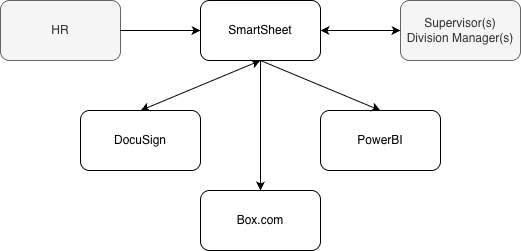
\includegraphics[width=\linewidth]{workflow.png}
    \caption{System Workflow Overview}
    \label{fig:workflow}
\end{figure}

\noindent
\textbf{Workflow Explanation}

The following describes the high-level data and process flow within the system:

\begin{enumerate}
    \item \textbf{HR -> Smartsheet} \\
    HR staff create or update records in Smartsheet to initiate workflows such as performance reviews, personnel matters, recruitment tracking, or employee separations.

    \item \textbf{Supervisors/Managers -> Smartsheet} \\
    Supervisors and managers review, update, and approve assigned records directly within Smartsheet.

    \item \textbf{Smartsheet -> Users (Email Notifications)} \\
    Automated notifications and reminders are sent to responsible users when actions are required or deadlines approach.

    \item \textbf{Smartsheet -> Automation Service (Python/AWS Lambda)} \\
    When required, workflow events trigger a cloud-based automation service to perform advanced processing tasks such as email generation, document handling, and cross-system synchronization.

    \item \textbf{Automation Service -> Box} \\
    Finalized documents are securely stored in Box, and the corresponding file links are written back to the appropriate workflow record.

    \item \textbf{Smartsheet -> Power BI} \\
    Workflow data is synchronized with Power BI to generate dashboards and reports for leadership visibility.

    \item \textbf{Box -> Authorized Users} \\
    Authorized users access finalized documents through secure Box links.
\end{enumerate}

% --------------------- Appendix C ---------------------
\section{To Be Determined (TBD) Items}

The following items remain to be finalized:

\begin{itemize}
    \item Final DocuSign field mappings and template identifiers.
    \item Box retention labels and document classification policies.
    \item Power BI workspace configuration and deployment settings.
    \item Detailed test cases and the finalized Requirements Traceability Matrix (RTM).
\end{itemize}

\end{document}

